\documentclass[thesis,fonts=libertine]{cluu}

\usepackage[style=cluu]{biblatex}
\usepackage{amsmath}

\DeclareMathOperator*{\argmax}{arg\,max}
\DeclareMathOperator*{\argmin}{arg\,min}

\usepackage{tikz}
\usepackage{graphicx}
\usepackage{url}
\usepackage{listings}
\usepackage{siunitx}
\usepackage[boxed, noline]{algorithm2e}
\usepackage{pgfplots}
\usepackage{pdfpages}

\graphicspath{ {figures/} }
\addbibresource{thesis.bib}

\usepackage{pythonhighlight}    % for \inputpython at the end

\begin{document}
\author{Shifei Chen}
\supervisors{Ali Basirat, Uppsala University}
\title{Cross-lingual Word Embeddings Beyond Zero-shot Machine Translation}

\maketitle

\begin{abstract}
  This thesis explored the possibility of transferring learning from training languages to completely unknown languages in a multilingual neural machine translation system. Using cross-lingual word embeddings as the only knowledge source, we observed little transferability from the training language to other completely unseen test languages. Also, the minor transferability only happens between highly-related languages from our experiment. The lack of regularization in our attentional encoder-decoder model caused the transformation of the output vector space and made it no longer aligned with the input vector space. Finally, to mitigate such architectural shortcomings of our multilingual translation model, we provided suggestions that could better share embedding layers from the training language to unknown languages.
\end{abstract}

\tableofcontents

\addchap{Preface}

This thesis was finished under the supervision of Ali Basirat. I would like 
to thank him first for his guidance, inspiration and passion.

The Saga supercomputer owned by UNINETT Sigma2 hosted all of the experiments in this thesis.\footnote{\url{https://www.sigma2.no/systems\#saga}} Without it this thesis would not be possible.

Thank you Mr. Anders Wall and everyone in the Anders Wall Scholarship Foundation for sponsoring my Master's study. This opportunity led me to meet everyone in the Master Programme in Language Technology, from whom I have learned a lot during the 2-years journey.

Last but not least, I would like to say a thank you to my parents for their unconditional love and support; to all of my friends for the unique memories we have created; and to my girlfriend, who has always been next to me when the virus made everything unusual.

% by using \addchap instead of \chapter this preface isn't numbered.

\chapter{Introduction}

Multilingual neural machine translation (NMT) aims to train a single translation model for multiple languages \parencite{Johnson:2016aa,aharoni-etal-2019-massively}. One of its appealing points is zero-shot translation, which enables translations between unseen language pairs when knowledge from one language is transferred to another language by the model's shared parameters. Even though both source and target languages in such an unseen pair should still be in the set of training languages, a multilingual NMT system with zero-shot learning is still attractive as it lowers the cost of obtaining expensive parallel data, particularly when translating low-resource languages.

The success of zero-shot translation depends on the model's ability to learn language invariant features \parencite{Arivazhagan:2019aa}. \textcite{Kim:2019aa} believes the embedding layers is one of the critical components responsible for learning such generalized features in a multilingual NMT system. By contrast, \textcite{aji-etal-2020-neural} concluded that sharing the embedding layer alone is not enough to transfer learning in zero-shot machine translation. No matter embedding layers are essential to zero-shot learning or not, they both showed that it would positively impact the multilingual model's transferability as long as the embeddings layers are aligned between the source language and the target language.

By far, researches on zero-shot learning in multilingual NMT have mostly been restricted to the limited scope of unseen language pairs. A majority of the previous studies of cross-lingual word embeddings in multilingual translation target zero-shot language pairs, not completely unseen languages. People exam on test sets whose languages on both the source or the target side of the translation are known to the system, but the paired combination remains unknown. For language pairs $A \rightarrow \text{EN}$ and $\text{EN} \rightarrow B$, they are all interested in the unseen language pair $A \rightarrow B$. There is less discussion about the multilingual NMT transferability on completely unknown languages that have never been in the training data.

This thesis studies the importance of word representation in the multilingual NMT transfer model based on the pre-trained cross-lingual word embeddings \parencite{Bojanowski:2016aa,Ammar:2016aa,Joulin:2018aa,Ruder:2019aa} and pushes it further than unseen language pairs --- examining the transferability of a multilingual NMT when it is applied to a new test language.

Despite the debate on whether cross-lingual word embeddings are vital when transferring information in zero-shot translation, it is generally acknowledged that cross-lingual word embeddings are beneficial for the model's transferability. Thus we will use cross-lingual word embeddings as the source of transfer knowledge to the test languages and leave the translation model's shared parameters to model the interrelationships between the training languages.

We train a multilingual neural machine translation model using cross-lingual word embeddings from high resource languages and test the translation quality on other languages that are unknown to the model. We hypothesize that a multilingual NMT model trained with pre-trained cross-lingual word embeddings should transfer reasonably even to a completely unknown language. Although from the experiment results, cross-lingual word embeddings transfer only marginally between closely related languages. Our findings are in line with \textcite{aji-etal-2020-neural} and indicate that some regularization is necessary to transfer the embedding layers between languages. Furthermore, when using cross-lingual word embeddings as the only transferable knowledge source, the performance will be negatively affected by the transformed output vector space, which needs to be countered in the future.

The rest of the thesis is organized as below:

Chapter \ref{chap:background} talks about the background and previous works when working in the transferability of cross-lingual word embeddings scope, including information about cross-lingual word embeddings and multilingual neural machine translation. After that, Chapter \ref{chap:method} introduces our experiment method, whose results are discussed and analyzed in Chapter \ref{chap:results}. Finally, Chapter \ref{chap:conclusion} gives out our conclusion. We also show sample outputs of our multilingual NMT model in Appendix \ref{chap:example_output}.

\chapter{Background}
\label{chap:background}

\section{Word Embeddings}
\subsection{Representing Words by Vectors}

In Natural Language Processing, people need to represent words in the forms that are more efficient for computers to process. The idea started with statistical language modeling, which was introduced to machine translation in the early nighties \parencite{brown-etal-1990-statistical}, followed by \textcite{bengio2003neural} who powered statistical language modeling with neural networks.

To turn words into vectors, one could use a simple one-hot encoding. For a vocabulary $V$ whose $|V|=n$, each word in the vocabulary can be uniquely represented in an $n$ dimensional vector consist of only one high value one and $n-1$ low value zeroes. Like in the example of $V=\{\text{water}, \text{hydrogen}, \text{oxygen}\}$ we could make $\vec{w}=[1, 0, 0]$, $\vec{h}=[0, 1, 0]$ and $\vec{o}=[0, 0, 1]$. However, these one-hot vectors cannot capture any latent semantic information between different words, nor to reflect the inflections between stems and their variants.

Recent vectorized word representations (word embeddings) were learned by neural networks. Compared to the naive one-hot vectors, word embeddings contains affluent information that links words together. They are able to transfer the semantical similarity between words to the similarity between vectors. Given two sentences with the target words \textit{oxygen} and \textit{hydrogen},

\begin{quotation}
  \textit{Oxygen} is a kind of gas.

  \textit{Hydrogen} is also a kind of gas.
\end{quotation}

\noindent the neural network would see from those similar context words and learn that the two target words \textit{oxygen} and \textit{hydrogen} have similar meanings. Hence it will produce two word embedding $\vec{o}$ and $\vec{h}$ with similar values, as seen in Figure \ref{fig:semantic_vectors}.

\begin{figure}
  \centering

  \tikzset{every picture/.style={line width=0.75pt}} %set default line width to 0.75pt

  \begin{tikzpicture}[x=0.75pt,y=0.75pt,yscale=-1,xscale=1]
  %uncomment if require: \path (0,256); %set diagram left start at 0, and has height of 256

  %Shape: Axis 2D [id:dp40983147480798976] 
  \draw  (-1,240.35) -- (210.5,240.35)(20.15,50) -- (20.15,261.5) (203.5,235.35) -- (210.5,240.35) -- (203.5,245.35) (15.15,57) -- (20.15,50) -- (25.15,57)  ;
  %Straight Lines [id:da060011766798584776] 
  \draw [color={rgb, 255:red, 80; green, 227; blue, 194 }  ,draw opacity=1 ][fill={rgb, 255:red, 182; green, 34; blue, 34 }  ,fill opacity=1 ]   (20.15,240.35) -- (102.58,195.85) ;
  \draw [shift={(104.34,194.9)}, rotate = 511.64] [color={rgb, 255:red, 80; green, 227; blue, 194 }  ,draw opacity=1 ][line width=0.75]    (10.93,-3.29) .. controls (6.95,-1.4) and (3.31,-0.3) .. (0,0) .. controls (3.31,0.3) and (6.95,1.4) .. (10.93,3.29)   ;
  %Straight Lines [id:da46956564149919644] 
  \draw [color={rgb, 255:red, 245; green, 166; blue, 35 }  ,draw opacity=1 ]   (20.15,240.35) -- (108.6,210.64) ;
  \draw [shift={(110.5,210)}, rotate = 521.4300000000001] [color={rgb, 255:red, 245; green, 166; blue, 35 }  ,draw opacity=1 ][line width=0.75]    (10.93,-3.29) .. controls (6.95,-1.4) and (3.31,-0.3) .. (0,0) .. controls (3.31,0.3) and (6.95,1.4) .. (10.93,3.29)   ;

  % Text Node
  \draw (92,220) node [anchor=north west][inner sep=0.75pt]    {$\vec{o}$};
  % Text Node
  \draw (69,185) node [anchor=north west][inner sep=0.75pt]    {$\vec{h}$};


  \end{tikzpicture}

  \caption{Illustraion of a vector space where $\vec{o}=\text{vec}(\text{oxygen})$ and $\vec{h}=\text{vec}(\text{hydrogen})$ are learned from two similar sentences.}
  \label{fig:semantic_vectors}
\end{figure}

Also, from a geometric prespective, we can observe a small angle between $\vec{h}$ and $\vec{o}$. From the cosine similarity definition,

\begin{equation*}
  \text{sim}(x, y) = \cos(\theta) = \frac{x \cdot y}{||x||||y||}
\end{equation*}

\noindent the smaller the angle $\theta$ between $\vec{h}$ and $\vec{o}$ is, the higher their cosine similarity is. In other words, when $\theta$ is zero, the cosine similarity $\text{sim}(x, y) \in [0, 1]$ will also approach its upper bound one.

 One of such algorithms to learn word embeddings from a large corpus of text is Word2Vec \parencite{Mikolov:2013aa,Mikolov:2013ab}, which learns word representations through a Skip-gram model or a Continuous Bag of Words (CBOW) model. Both models are shown in Figure \ref{fig:skip_gram_and_cbow} and they have been continuously driving other word embedding algorithms such as fastText \parencite{Joulin:2018aa}.\footnote{\url{https://fasttext.cc/docs/en/unsupervised-tutorial.html}}

\begin{figure}
  \centering
  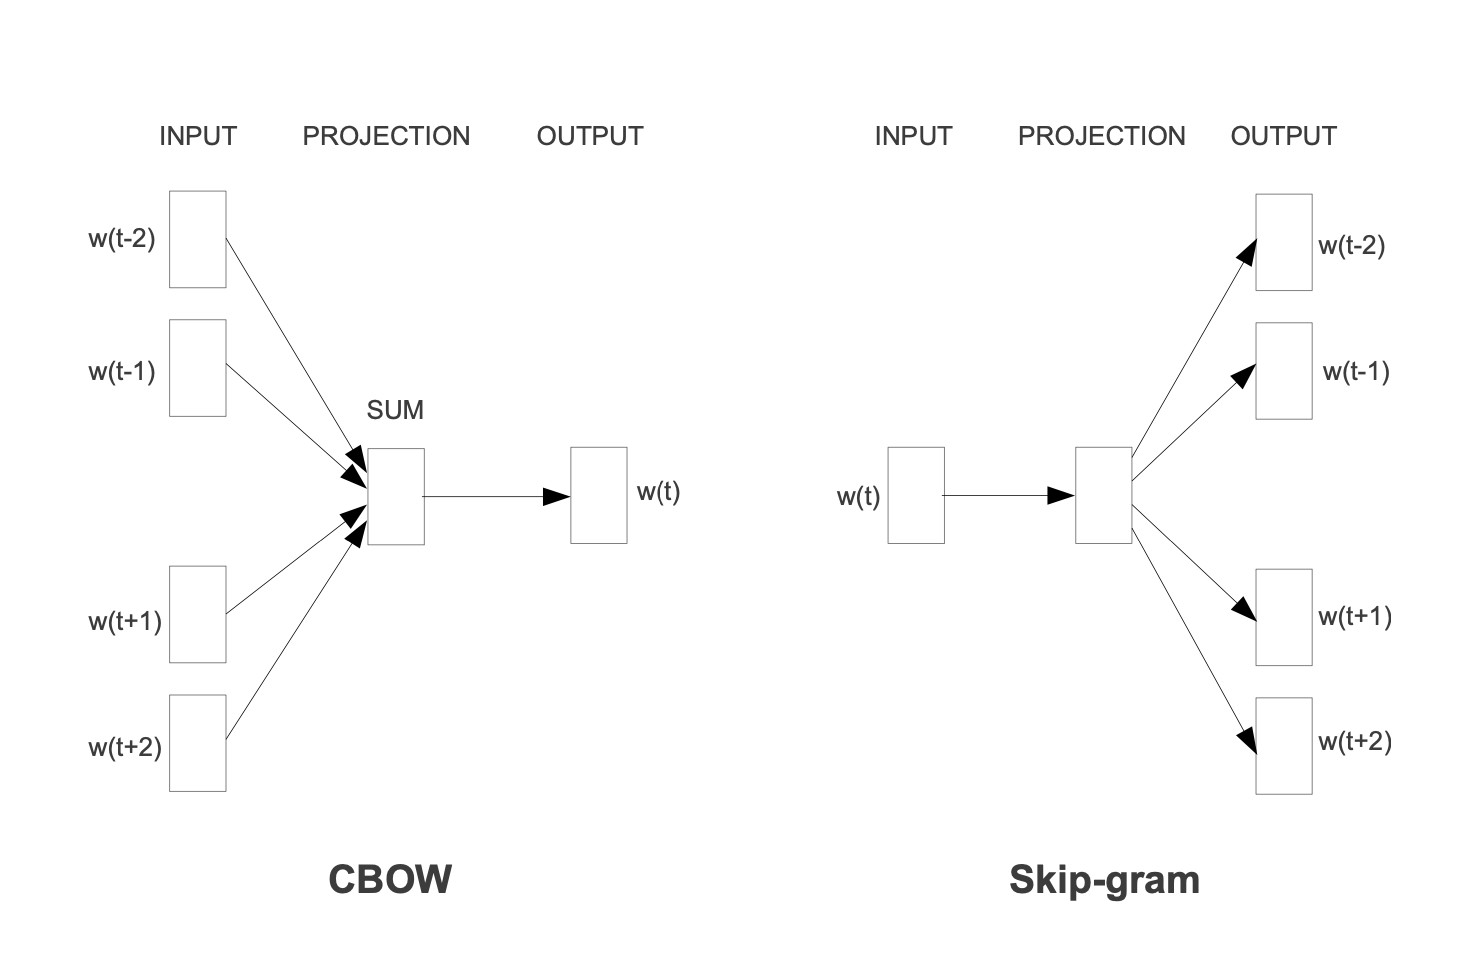
\includegraphics[width=0.8\textwidth]{skip_gram_and_cbow_models.png}
  \caption{The Skip-gram and the CBOW model \parencite{Mikolov:2013ac}. The Skip-gram model predicts contextual words based on the given center word, while the CBOW model predicts the center word from given context words.}
  \label{fig:skip_gram_and_cbow}
\end{figure}

\subsection{Cross-lingual Word Embeddings}
\label{sec:multilingual_word_embeddings}

Learned from approaches like the Skip-gram model or the CBOW model, vectorized word representations tend to cluster words with similar semantics \parencite{Mikolov:2013ac}. It then becomes attractive to see whether we could fit two or more languages into the same vector space. Multilingual word embeddings in the same vector space are called cross-lingual word embeddings.

\begin{figure}
  \centering
  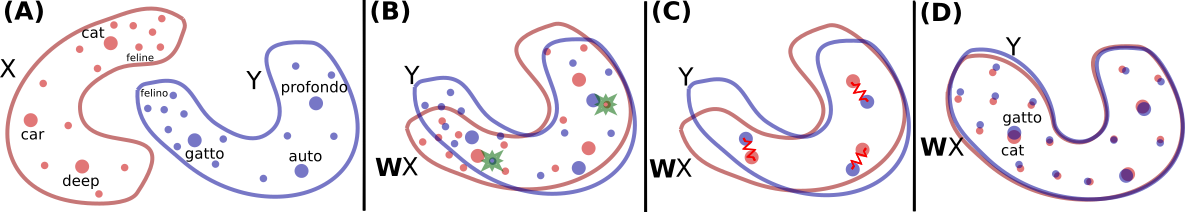
\includegraphics[width=0.8\textwidth]{vector_spaces_alignment.png}
  \caption{Aligning bilingual vector spaces. \parencite{Conneau:2017aa}}
  \label{fig:vec_space_align}
\end{figure}

In the multilingual scenario, alignment in two different vector spaces is vital in order to make word embeddings from different languages comparable. Figure \ref{fig:vec_space_align} illustrated the alignment method from \textcite{Conneau:2017aa}. Suppose there is a set of word pairs $\{x_i, y_i\}$ where ${i\in \{1, ..., n\}}$, the two vector spaces were aligned by a rotation matrix $W \in \mathbb{R}^{d \times d}$ as shown in process \textbf{(B)}, to optimize the objective function 

\begin{equation*}
  \min_{W \in \mathbb{R}^{d \times d}} \frac{1}{n}\sum_{i=1}^n \ell(Wx_i, y_i)
\end{equation*}

\noindent Here $\ell$ is the loss function and it is usually the square loss function $\ell(x, y)=||x-y||^2$. Then $W$ is further refined in process \textbf{(C)}, where we choose frequent words as anchor points and minimize the distance between each correspondent anchor points by an energy function. After this, the refined $W$ is then used to map all words in the dictionary during the inference process. We obtain the translation $t(i)$ of a given source word $i$ in the formula

\begin{equation*}
  t(i) = \argmin_{j\in \{1, ..., N\}} \ell(Wx_i, y_j)
\end{equation*}

In practice, people use lexicon as the most common parallel data to learn the alignment of multiple vector spaces, though there are other kinds of alignment using sentence or documents level data \parencite{Ruder:2019aa}. By using word-level information like a dictionary, we can start with a pivot language (usually English) and map each other monolingual word embeddings by looking the same word up in the dictionary \parencite{Mikolov:2013ac}. Sentence-level parallel data usually contains aligned sentence pairs from different languages \parencite{Hermann:2013aa}. Document-level information is usually a group of topic-aligned or class-aligned documents, such as articles from the same Wikipedia item in different languages \parencite{vulic-moens-2013-study}.

Recent development in word alignment has shown possibilities for less supervision and smaller seed data size to initiate the alignment process \parencite{Ruder:2019aa}. Though it is still unclear if cross-lingual word embedding alignment can run without parallel data or supervision \parencite{Dyer1365879}, there is evidence that even word embeddings from distant language pairs have similar geometric arrangements in vector spaces \parencite{Mikolov:2013ac}.

\section{Multilingual Neural Machine Translation (NMT) Systems}

\subsection{Multilingual Neural Machine Translation}

Neural Machine Translation (NMT) uses neural networks to learn the translation relationship between a source and a target language. It has outperformed the traditional statistical machine translation in some machine translation settings and has enabled some new possibilities in the field. One of these new applications is multilingual NMT. As shown in Figure \ref{fig:google_mnmt}, the system has an encoder and a decoder consisting of several layers of LSTM network spread parallelly on multiple GPUs. An attention module serves as the connection bridge between the encoder and the decoder. It emphasizes which part of the source sentence is more relevant to the current translation context, especially when translating long sentences \parencite{Wu:2016aa}. Multilingual NMT uses the same attentional encoder-decoder model but trains it on a multilingual corpus with additional artificial tokens to indicate the target language \parencite{Johnson:2016aa}.

\begin{figure}
  \centering
  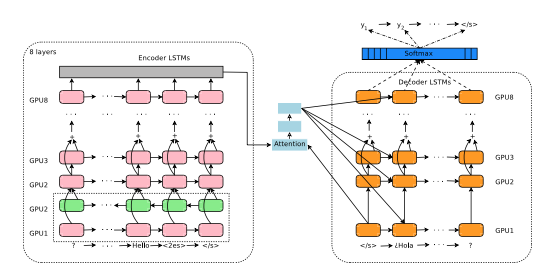
\includegraphics[width=0.8\textwidth]{google_mnmt_architecture.png}
  \caption{Google's MNMT Architecture \parencite{Johnson:2016aa,Wu:2016aa}}.
  \label{fig:google_mnmt}
\end{figure}

The benefit of such a multilingual NMT system does not necessarily stop at better translation performance between common languages like English, French, or Spanish; it also leverages additional information from high resource languages to low resource languages, as a special form of transfer learning \parencite{Zoph:2016aa}.

\textcite{Lakew:2019aa} claim such form of transfer learning may happen both in the horizontal or vertical direction: In the horizontal direction, knowledge transfers from pre-trained data (such as word embeddings or language models) and is fine-tuned on the test data in known languages; in the vertical direction, knowledge transfers from known language pairs to the test data in an unknown language.

In our experiments, we use information from our training languages and examine its transferability to the unseen test language. We do not apply any fine-tuning based on our test data and keep our test data entirely untouched by the multilingual NMT model. Our Methodology is thus vertical transfer learning, the same as zero-shot machine translation.

\subsection{Zero-shot Machine Translation}
\label{sec:zero_shot_mt}

Zero-shot translation stands for translation between language pairs invisible to the multilingual NMT system during the training time. For example, building a multilingual NMT system with German-English and French-English training language pairs while testing its performance on a German-French scenario. In 2016, \textcite{Johnson:2016aa} first published their result on a zero-shot MT system. Their multilingual MT system includes an encoder, a decoder, and an attention module. It requires no change to a standard NMT system except introducing an additional token at the beginning of each source sentence to denote the translation target language. \textcite{Ha:2016aa} also showed that their universal encoder and decoder model is capable of zero-shot MT. Translation between unseen language pairs is attractive, especially for low-resource language pairs. Compared with a pivot based system, zero-shot translation eliminates the need for a bridging language, or \textit{interlingua}, as an intermediary of the source and target language. However, zero-shot translation still underperforms than pivot-based translation.

Two reasons could explain the gap between a zero-shot system and a pivot based system, language bias \parencite{Ha:2016aa, Ha:2017aa, Arivazhagan:2019aa} and poor generalization \parencite{Arivazhagan:2019aa}. Language bias means that the MT system tends to decode the target sentence into the wrong language during inference, usually copying the source language or the bridging language \parencite{Ha:2016aa}. It could be the consequence of always translating all source languages into the bridging language, making the model difficult to learn to translate to the desired target language \parencite{Arivazhagan:2019aa}.

The other potential reason for the worse performance of a zero-shot system is poor generalization. When a zero-shot system is trained purely on the end-to-end translation objective, the model prefers to overfit the supervised translation direction features than learn more transferable language features. There is no guarantee that the model would discover language invariant representations as there is no explicit incentive to learn language invariant features, resulting in the intermediate encoder representations are too specific to individual languages \parencite{Arivazhagan:2019aa}.

To fix these two problems, there has been work on improving the preprocessing process \parencite{Lakew:2018aa}, parameter sharing \parencite{Firat:2016aa, Blackwood:2018aa}, additional loss penalty functions \parencite{Arivazhagan:2019aa} and pre-training modules using external information \parencite{Baziotis:2020aa}. In some of the improvements, zero-shot system could achieve better performance than pivot based systems.

\section{Cross-lingual Word Embeddings in Multilingual NMT}

In terms of the application of cross-lingual word embeddings in a multilingual NMT system, there are some successful applications such as using the cross-lingual word embeddings as the embedding layer \parencite{neishi-etal-2017-bag, Artetxe:2017aa}, as the substitution of a supervised dictionary \parencite{Conneau:2017aa}, or as an external supplementary extension \parencite{inproceedings}. There are even cases where people successfully trained an MT system using very little or none parallel data \parencite{Conneau:2017aa} and heavily rely on cross-lingual word embeddings. 

\textcite{Qi:2018aa} look at cross-lingual word embeddings and their performance in a multilingual setting in detail. They find that cross-lingual word embeddings are useful in a multilingual NMT system, while in bilingual NMT systems, pre-trained word embeddings do not necessarily need to be aligned. \textcite{Qi:2018aa} attribute the BLEU score increase to the architecture design of the attentional encoder-decoder multilingual NMT system. As such multilingual NMT system uses a single encoder for all source languages, alignment in the word embeddings condenses various vector spaces of the source language into a unified vector space, helping the system learn a much-simplified transform from its input vector space to its output vector space.

\chapter{Methodology}
\label{chap:method}

\section{Experiment Settings}
\label{sec:initial_exp_settings}

We chose English (EN), German (De), and French (FR) to be the training languages as these three languages are all considered to be high-resource languages. Selecting them as our training languages would enable a wider choice of available training resources for our experiments.

Let $Z$ denote the set of corresponding candidate languages, the training language set is then $Z_{TRAIN} = {\text{EN}\cup \text{DE}\cup \text{FR}}$. For the test language set, we picked up Swedish (SV) as a low-resource language representation within the same language family of our training languages, Hungarian (HU), and Hebrew (HE) as another two low-resource language examples that do not belong to the same language group as our training languages. Therefore $Z_{TEST} = {\text{SV}\cup \text{HU}\cup \text{HE}}$.

For each experiment, we trained a basic multilingual NMT system using a training corpus $C_{TRAIN}$ with all three training languages, including all six combinations from the cartesian product without duplicates. Here $x$ and $y$ are both training languages in the training set $C_{\text{TRAIN}}$.

\begin{equation*}
  C_{\text{TRAIN}} = \{x \times y \mid x, y \in Z_{\text{TRAIN}} \text{ and } x \neq y\}
\end{equation*}

During testing, the multilingual NMT system is tested on the test corpus with all three training languages and one of the test language. The test corpus consists of both translation directions of three different training language and that only test language.

\begin{equation*}
  C_{\text{TEST}} = \{(x, y)\cup(y,x) \mid x \in Z_{\text{TRAIN}} \text{ and } y \in Z_{\text{TEST}}\}
\end{equation*}

We use BLEU \parencite{papineni-etal-2002-bleu} as one of our evaluation metrics, together with 1-4 word gram precision scores to better understand if the transferability only happens at word level or at phrase level.

\subsection{Corpus and Preprocessing}

we use the TED talk subtitle corpus from \textcite{Qi:2018aa} to train the multilingual NMT.\footnote{\url{https://github.com/neulab/word-embeddings-for-nmt}} The whole corpus is split into three parts, train, dev, test at the ratio of $0.95:0.025:0.025$.

For preprocessing, since the original TED corpus is already tokenized by Moses \parencite{koehn-etal-2007-moses}, we did not add additional tokenization steps. We turned all of the text into lower cases and applied a sentence length filter to remove all long sentences with more than 60 words. After that, when building the index to word (i2w) and the word to index (w2i) table for the pre-trained embeddings, we have also removed words that are less frequent than two times to stop the system from overfitting by low-frequency words.

All of the preprocess functions are built upon the built-in XNMT preprocess features \parencite{Neubig:2018aa}. Table \ref{table:preprocessing} contains the corpus size for all of the training and test language sets.

\begin{table}
  \centering
  \begin{tabular}{r|rrr}
    \hline
    \textbf{Language} & \textbf{train} & \textbf{dev} & \textbf{test} \\ [0.25ex]
    \hline\hline
    EN+DE+FR & 1013478 & N/A & N/A \\
    +SV & N/A & 9390 & 12423 \\
    +HU & N/A & 20332 & 25606 \\
    +HE & N/A & 24554 & 28546 \\
    \hline
    EN+DE+DA & 491537 & N/A & N/A \\
    +SV & N/A & 8037 & 9344 \\
    \hline
    EN+DE+DA+NL & 1225511 & N/A & N/A \\
    +SV & N/A & 11126 & 13378 \\
    \hline
    EN+DE+DA+NL+NO & 1322133 & N/A & N/A \\
    +SV & N/A & 12304 & 14430 \\
    \hline
  \end{tabular}
  \caption{Number of sentences in each language combination after preprocessing}
  \label{table:preprocessing}
\end{table}

\subsection{Neural Network}

Our neural network is a modified version of the one from \textcite{Qi:2018aa}, which is built with XNMT \parencite{Neubig:2018aa}. The only change is doubling the encoding layer to a 2-layer-bidirectional LSTM network, thus having more parameters to accommodate the additional information in a multilingual scenario. Everything else is the same as the original experiment settings: we set the beam size to $5$, the batch size to $32$ and the dropout rate to $0.1$. The optimizer used in our experiments is the Adam Optimizer \parencite{Kingma:2014aa}. We use BLEU score \parencite{papineni-etal-2002-bleu} as well as 1-4gram precision scores as our evaluation metrics. The initial learning starts at $0.0002$ and decays by $0.5$ when the development BLEU score decreases \parencite{Denkowski:2017aa}.

\subsection{Embeddings}

The embeddings used in the experiments are fastText aligned word embeddings.\footnote{\url{https://fasttext.cc/docs/en/aligned-vectors.html}} They are based on the pre-trained vectors on Wikipedia using fastText \parencite{Bojanowski:2016aa}.\footnote{\url{https://www.wikipedia.org/}} The alignment is performed using RCSLS as in \textcite{Joulin:2018aa}.

fastText is an extension of the original Word2Vec methods, which uses sub-words to augment low-frequency and unseen words. It also has an extensive collection of pre-trained embeddings for multiple languages out of the box, making it attractive to cross-lingual word embedding experiments like ours since researchers can save effort on training and aligning cross-lingual word embeddings while concentrating on experiments themselves.

Each of the fastText word embedding file is language-specific and contains word embeddings in 300 dimensions. We concatenated different language files to build up cross-lingual word embedding files for the multilingual NMT system. The embeddings are frozen during the whole training to remain the original alignment throughout the whole experiments. If there is a shared word with two different vector values in different language embedding files, both vectors' average value will be used.

There will also be a different attempt in our experiments where the system treats each word as a unique word even though they might share the same spelling. Both of the results will be available below in Section \ref{sec:langauge_similarity}.


\chapter{Results and Analysis}
\label{chap:results}

\begin{table}
  \centering
  \begin{tabular}{r|*{5}{l}}
    \hline
    \textbf{Language} & \textbf{BLEU} & \textbf{1gram} & \textbf{2gram} & \textbf{3gram} & \textbf{4gram} \\ [0.25ex]
    \hline\hline
    EN+DE+FR & 29.22 & 0.57 & 0.34 & 0.24 & 0.16 \\
    SV & 1.12 & 0.16 & 0.02 & 0.00 & 0.00 \\ 
    HU & 1.12 & 0.18 & 0.02 & 0.00 & 0.00 \\
    HE & 1.02 & 0.16 & 0.02 & 0.00 & 0.00 \\
    \hline
  \end{tabular}
  \caption{Initial results for SV, HU and HE on the baseline system (Target language annotation only, dropout=0.3, trained on mixed language branch corpus.)}
  \label{table:initial_results}
\end{table}

Table \ref{table:initial_results} shows our initial result from a multilingual machine translation model trained on the combined EN+DE+FR corpus. Swedish, Hungarian and Hebrew all got unanticipated low BLEU scores. Unlike the reported results from \textcite{Qi:2018aa}, even though Swedish is closer to the training languages, the expected high performance based on its high similarity to the training languages did not appear in our experiment result. All of the three languages only achieved around 1 BLEU score. Also, since the system hardly translates any of the languages, it is hard to tell the relationship between language similarity and the model's performance. However, when it comes to randomly initialized embedding layers without pre-trained embeddings, cross-lingual word embeddings still provides better initialization than random settings. We see the translation model trained with cross-lingual embeddings performs substantially better (Avg BLEU=1.2) than a model trained with randomly initialized embeddings (BLEU=0.1).

By looking at individual 1-4 gram precision scores, all three languages had a significantly better unigram precision score than their bigram, trigram, and quadgram precision score. For example in Swedish, its bigram precision score in Swedish was about half of its unigram scores. The precision score on trigrams and quadgrams are close to zero on all languages, which again is a sign showing the multilingual NMT system has little transferability from known training languages to an unknown test language, and that transferability only happens at word level.

We have tried increasing the dropout rate to 0.3 and observed small improvements (average 0.5 BLEU score increase). As \textcite{Arivazhagan:2019aa} have pointed out, this technique improves the zero-shot performance at the cost of supervised translation directions. Thus we decided to explore other approaches below.

\section{The Effect of Language Similarity}
\label{sec:langauge_similarity}

In the above results from Table \ref{table:initial_results}, even though all of the BLEU scores from three test languages are relatively low, Swedish achieves the best result. To better understand whether and how Swedish benefits from its language similarity to our training languages, we have further designed experiments to see the effect of language similarity.

The additional experiments will still use Swedish as the test language while removing French as the training language to homogenize the training language set more towards Swedish. In the previous training language set, French is the only training language that is Romanic. By replacing French with Danish, all of the training languages are now Germanic, as well as the test language Swedish. We have also included two more Germanic languages to the training language set, Dutch (NL) and Norwegian (NO). We began with an experiment trained on English, German and Danish, and added the additional training languages one by one in the next two experiments. Everything else is the same. The results are shown in Table \ref{table:language_similarity}.

\begin{table}
  \centering
  \begin{tabular}{r|*{5}{l}}
    \hline
    \textbf{Language} & \textbf{BLEU} & \textbf{1gram} & \textbf{2gram} & \textbf{3gram} & \textbf{4gram} \\ [0.25ex]
    \hline\hline
    EN+DE+FR & 1.12 & 0.16 & 0.02 & 0.00 & 0.00 \\
    \hline
    EN+DE+DA & 4.1 & 0.28 & 0.07 & 0.02 & 0.01 \\
    +NL & 3.3 & 0.23 & 0.05 & 0.02 & 0.00 \\ 
    +NO & 4.7 & 0.31 & 0.07 & 0.03 & 0.01 \\
    \hline
  \end{tabular}
  \caption{Results for language similarity tested on the Swedish language. Three other Germanic languages DA, NL and NO were added one by one into the training corpus.}
  \label{table:language_similarity}
\end{table}

As the results show, the system gained the most improvements when Danish and Norwegian were added. Although Dutch does not help the multilingual NMT system learn how to translate from Swedish or into Swedish a lot, compared with the original baseline EN+DE+FR experiment, adding Dutch in the training language still increases the BLEU score by more than 2 points. The result from our language similarity experiments confirms that close languages would benefit each other more than distant languages in a multilingual NMT system using pre-trained cross-lingual word embeddings \parencite{Qi:2018aa}.

Swedish, Danish and Norwegian have deep historical relationships with each other. Therefore, these languages share many vocabularies as well as grammar and syntax rules. To study how much of such kind of benefit was brought by shared vocabularies or similar syntax, we conducted a further experiment by differentiating the word origin as below: each word in the training corpus was tagged by its source language token to distinguish its origins. Punctuations are not distinguished among languages, which means they do not receive a language-specific token. Word embeddings are also tagged to point to the correct source words. A Swedish sentence that needs to be translated into German is then

\begin{verbatim}
  __de__ <<sv>>och <<sv>>vi <<sv>>kämpar <<sv>>med <<sv>>dem .
\end{verbatim}

The assumption behind the word origin token is that, if the result suffers when each word differs by its origin language, the multilingual NMT system would primarily translate by shared vocabularies between languages; if its results still hold after the modification, it would primarily learn translation from information other than shared vocabularies.

The system has obtained a 1.7 BLEU score on the EN+DE+DA to SV experiment. It showed that if each word is no longer allowed to be shared between languages, the models' performance would dramatically decrease. Hence most of the improvements were brought by the fact that Swedish, Danish and Norwegian have a large number of common vocabularies. On the other side, it also indicates that the system did not learn too much non-vocabulary information during training, e.g., similar grammar structures. Otherwise, we would see a smaller BLEU score gap between the results as such non-vocabulary information will be preserved in the embedding layer. We conclude that our multilingual NMT system here primarily learns lexicon translation.

\section{The Effect of the Transformed Vector Space}

In addition to the role of language similarity between the training languages and the test languages, we also hypothesize that our multilingual NMT model's poor transferability to unseen languages is due to transformed vector space in the translation model. After a series of linear operations from the neural network onto the word embeddings, the output vector space is no longer aligned with the input vector space. Before our experiments, we predicted that our NMT system should have learned the generally mapping between words in the source vector space and the ones in the target vector space, even though the system has not seen the correct word in the target word space during training.

However, by looking closely at the output translation in Table \ref{table:initial_results}, we have observed the contrary --- almost none of the words in the output text are translated to the correct word in the desired languages. They were either incorrectly translated into one of the training languages, or were entirely copied from the source text. The BLEU score gains were from punctuations and a small collection of words shared between languages (e.g., property nouns).

Taking a step further, when analyzing both translation directions, there are other traces to support our transformed vector space suspicion. We have conducted comparisons in both directions on the Swedish language experiment, as shown in Table \ref{table:directional_results}. When translating from SV to the combined EN+DE+DA text, we could achieve almost 6 BLEU scores, which is much better than the nearly zero score when translating from the other direction. Also, compared to the combined precision scores on the same experiment from Table \ref{table:language_similarity}, the results of the translation direction EN+DE+DA $\rightarrow$ SV contributed almost nothing to the combined translation performance. We present the sample output of both directions in Appendix \ref{sec:directional_output}.

\begin{table}
  \centering
  \begin{tabular}{r|*{5}{l}}
    \hline
    \textbf{Language} & \textbf{BLEU} & \textbf{1gram} & \textbf{2gram} & \textbf{3gram} & \textbf{4gram} \\ [0.25ex]
    \hline\hline
    EN+DE+DA $\rightarrow$ SV & 0.65 & 0.14 & 0.01 & 0.00 & 0.00 \\
    SV $\rightarrow$ EN+DE+DA & 6.00 & 0.33 & 0.08 & 0.03 & 0.01 \\
    \hline
  \end{tabular}
  \caption{Results for individual translation direction between EN+DE+DA and SV.}
  \label{table:directional_results}
\end{table}

Thus, the model's decoder's output vectors may have been altered and are no longer in the same vector space as the input word embeddings. In this case, the transformed vector space has also made less sense to search for the correct word vector neighbors close to the predicted output vector in the output vector space. However, there opens a new possibility to translate from completely unknown languages to known languages. We could perform a lexicon replacement based on the Euclidean distance between words in the unknown language and one of the known languages, then feed the processed text into a translation model that has already been trained on known languages. During the whole process, the unknown language remains untouched by the translation model. Therefore it still qualifies as zero-resource translation. We will discuss the lexicon replacement process below.

\subsection{Lexicon Replacement By Euclidean Distance}

Suppose we have a vector space $S$ that contains cross-lingual word embeddings in the unknown language and the known languages, respectively. We donate them as $W_x$ and $W_k$. For each $w_x\in W_x$, there exists at least one mapping to a target word in the known languages $w_k \in W_k$. We are looking for that specific $w_k$ that is within a specific radius of the original $w_s$. The distance should still be relatively small so that $w_s$ and $w_k$ are considered an adequate translation of each other.

In theory, to determine the nearby neighbor $w_k$, we can use different kinds of metrics. Here we have chosen to use the Euclidean distance where determines the distance between $w_s$ and $w_k$ as

\begin{equation}
  d(w_s, w_k)=\sqrt{\sum_{i=1}^n{(w_{s_i}-w_{k_i})}^2}
\end{equation}

The distance $d$ is a variable here and its value needs to be determined as well. Hence there are experiments to test the distance argument $d$ by different experiments, ranging from $d=0.25$ to $d=5$.

The algorithm is described in Algorithm \ref{algo:subsitution}.

\begin{algorithm}[h]
  \SetAlgoLined
  \KwIn{hypothesis $H$, source language embeddings $E_s$, target language embeddings $E_t$, distance threshold $D$}
  \KwResult{Updated hypothesis $H^\prime$ with words being replaced by their neighbors in the desired language}

  Build kd-tree $T$ from $E_s$
  \For(each line $l$ in the source hypothesis $H$){$l \in H$}{
    \For(each word $w$ in line $l$){$w \in l$}{
      \uIf{$w$ is a punctuation}{
        skip $w$\;
      }
      \uElseIf{$w$ is an unknown word}{
        skip $w$\;
      }
      \Else{
        query distance $d(w, w^\prime)$ for $w$ in $T$\;
        \If{$d<D$}{
          replace $w$ with the correspoding $w^\prime$
        }
      }
    }
  }
  \caption{Pesudo code for output hypothesis word substitution. Each word in the NMT output hypothesis that is not in the desired language will be replaced by its closest neighbor in that language.}
  \label{algo:subsitution}
\end{algorithm}

Performing a distance query on a vector space with more than $\num{3e6}$ vectors is slow, especially when all these vectors are considered high dimensional vectors. The code was implemented with SciPy \parencite{Virtanen:2019aa}. There are algorithms like KD-tree \parencite{Maneewongvatana:aa} that could reduce the calculation time for low-dimensional vectors, but for vectors higher than 20 dimensions, it is not necessarily faster than brutal force.\footnote{As described on the API document, ``High-dimensional nearest-neighbor queries are a substantial open problem in computer science.'', \url{https://docs.scipy.org/doc/scipy/reference/generated/scipy.spatial.KDTree.html}} On the other hand, based on the Johnson–Lindenstrauss theorem \parencite{johnson1984extensions}, a vector space should have at least more than 300 dimensions to distinguish $\num{1e6}$ vectors in it. As the aligned vector space in fastText contains more than $\num{3e6}$ words, the dimensions could not be compressed anymore, or we are at risk of not be able to distinguish each word. After all, the script is slow at substitute every word in the output hypothesis into the corresponding one in the desired language.

We have performed the lexicon replacement experiment on the SV $\leftrightarrow$ EN+DE+DA text from the same TED text corpus \parencite{Qi:2018aa}, fed into an already trained translation model based on the NO $\leftrightarrow$ EN+DE+DA corpus, using NO as the pivot language. When applying the previously mention Algorithm \ref{algo:subsitution} on the SV $\leftrightarrow$ EN+DE+DA text, we replace all of the source text started without the target language token \verb|__SV__|. In other words, we translate all of the source sentences in Swedish to Norwegian first, leaving all of the other source sentences (sentences in EN, DE or DA) untouched. The target translation reference also remains as is. 

The BLEU scores are shown in Table \ref{table:lexicon_replacement}. To demonstrate the difference of applying the same algorithm on the input and the output vector space, we have also selected results from $d=0$ to $d=4$ and compared them with the results when Algorithm \ref{algo:subsitution} was performed on the output vector space. The comparison is in Figure \ref{fig:lexicon_replacement}.

\begin{table}
  \centering
  \begin{tabular}{r|*{5}{l}}
    \hline
    \textbf{$d$ value} & \textbf{BLEU} & \textbf{1gram} & \textbf{2gram} & \textbf{3gram} & \textbf{4gram} \\ [0.25ex]
    \hline\hline
    SV $\leftrightarrow$ EN+DE+DA & 4.1 & 0.28 & 0.07 & 0.02 & 0.01 \\
    \hline
    No replacement & 2.99 & 0.27 & 0.05 & 0.02 & 0.00 \\
    0.25 & 2.99 & 0.27 & 0.05 & 0.02 & 0.00 \\
    0.5 & 2.99 & 0.27 & 0.05 & 0.02 & 0.00 \\
    1 & 6.18 & 0.34 & 0.10 & 0.04 & 0.01 \\
    2 & 6.17 & 0.34 & 0.10 & 0.04 & 0.01 \\
    3 & 6.17 & 0.34 & 0.10 & 0.04 & 0.01 \\
    4 & 6.17 & 0.34 & 0.10 & 0.04 & 0.01 \\
    0 & 6.00 & 0.33 & 0.08 & 0.03 & 0.01 \\
    \hline
  \end{tabular}
  \caption{Results for the lexicon replacement experiments with different $d$ thresholds. Tested on SV text using NO as the pivot language on the NO $\leftrightarrow$ EN+DE+DA translation model. $d=0$ stands for no threshold control (replace every word).}
  \label{table:lexicon_replacement}
\end{table}

\begin{figure}
  \centering
  \resizebox{0.7\columnwidth}{!}{%
    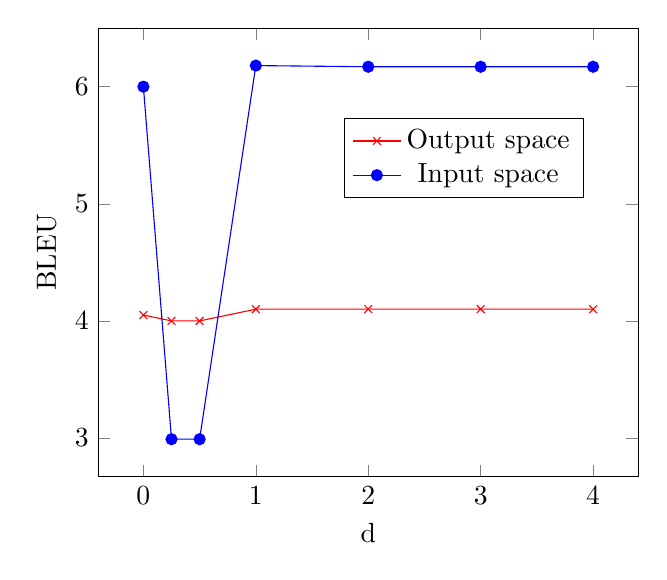
\begin{tikzpicture}
      \pgfplotsset{
        every axis legend/.append style={
          at={(0.9,0.8)},
          anchor=north east,
        },
      }
      \begin{axis}[
        xlabel=d,
        ylabel=BLEU]
        \addplot[color=red,mark=x] coordinates {
          (0,4.05)
          (0.25,4.0)
          (0.5,4.0)
          (1,4.1)
          (2,4.1)
          (3,4.1)
          (4,4.1)
        };
        \addplot[color=blue,mark=*] coordinates {
          (0,6.00)
          (0.25,2.99)
          (0.5,2.99)
          (1,6.18)
          (2,6.17)
          (3,6.17)
          (4,6.17)
        };
        \legend{Output space, Input space}
      \end{axis}
    \end{tikzpicture}
  }
  \caption{BLEU scores for the lexicon replacement algorithm applied on both the input and the output vector space.}
  \label{fig:lexicon_replacement}
\end{figure}

From both Table \ref{table:lexicon_replacement} and Figure \ref{fig:lexicon_replacement}, we can see a noticeable improvement over the baseline result as the BLEU score doubled. Even compared with the SV $\leftrightarrow$ EN+DE+DA model, the lexicon replacement experiment's result is still leading ahead for about 2 BLEU scores. Thus it demonstrates that our lexicon replacement hypothesis is effective within the input vector space.

Moreover, the value of $d$ will affect the translation model. As we increase $d$ from $0.5$ to $1$, we see a significant translation quality improvement. On the other side, increasing $d$ after $d=1$ will have no positive impact on the model's performance. When we set $d=0$ to remove the threshold control, its performance dropped around $0.2$ points, mostly due to the lowered bigram precision score. We conclude that there is a sweet spot for the $d$ value. Its accurate value needs to be fine-tuned to adapt to different source and pivot language combinations.

Finally, when comparing the results of lexicon replacement on the input vector space and the output vector space results, we confirmed the output vector space did change during the translation training process by the model's neural network. Unlike the input vector space, executing lexicon replacement on the output space does not have a leap on the BLEU score, no matter how the distance threshold $d$ changes. Hence it is not worth performing operations like lexicon replacement on the output vector space.

\chapter{Conclusion and Future Work}
\label{chap:conclusion}

In this thesis, we have explored the transferring and generalizability of cross-lingual word embeddings on unknown languages. From the achievement of zero-shot machine translation, we took a step further and expected moderate performance from those word embeddings as if they would transfer knowledge learned from the test languages onto other completely unknown languages. However, our experiment results suggested that only slight knowledge transfer happened between closely related languages, which echoes back to some of the findings that the embedding layer along in a multilingual NMT system is not enough to handle the knowledge transfer \parencite{aji-etal-2020-neural}.

To increase cross-lingual word embeddings' transferability in a multilingual NMT architecture similar to \textcite{Johnson:2016aa}, there should be some additional alignment in the output vector space between the source and the target languages. During the training process, the neural network has never seen any positive examples from the test language. Therefore its output weight on the test language has been continuously deducted, which resulted in a transformed output vector space. Such output space is no longer aligned with the input vector space, hence connections between different languages solely rely on shared vocabularies. As a result, only very similar languages such as Swedish, Norwegian and Danish benefited in our experiments.

As we have demonstrated in our lexicon replacement experiments, a solution to align the deviated input and output embedding spaces is to add regularization to the multilingual model's loss function based on the two vector spaces' divergence. Another potential solution to be explored is to supplement the translation model with language level information such as language embeddings \parencite{littell-etal-2017-uriel,malaviya-etal-2017-learning} together with the cross-lingual embeddings. Language level information could also answer more questions remained in our study. Together with some previous studies \parencite{Qi:2018aa,aji-etal-2020-neural}, we believe the transferability of cross-lingual word embeddings is related to the similarity between the source and the target language, but how to measure the language similarity and link it to the transferability of the embedding layers could be an exciting topic.

Finally, it is worth exploring how other sets of embeddings would enhance cross-lingual word embeddings' transferability. For example, to try the multilingual contextualized cross-lingual embeddings \textcite{devlin-etal-2019-bert} and see if it would benefit the transferability by adding contextual information, or the multilingual sub-word embeddings \textcite{Heinzerling:2017aa} if it would perform better by aligning more words between different languages.

\appendix
\chapter{Example Output from the Multilingual NMT Model}
\label{chap:example_output}

\section{Example Output from the Directional Translation Experiment}
\label{sec:directional_output}

This sample output is taken from the SV $\leftrightarrow$ EN+DE+DA experiment, described in Section \ref{sec:langauge_similarity}. Its perfromance result is in Table \ref{table:language_similarity}.

We have sampled 20 sentences from the output file. Each of the languages (SV, EN, DE and DA) as the target translation language has five examples.

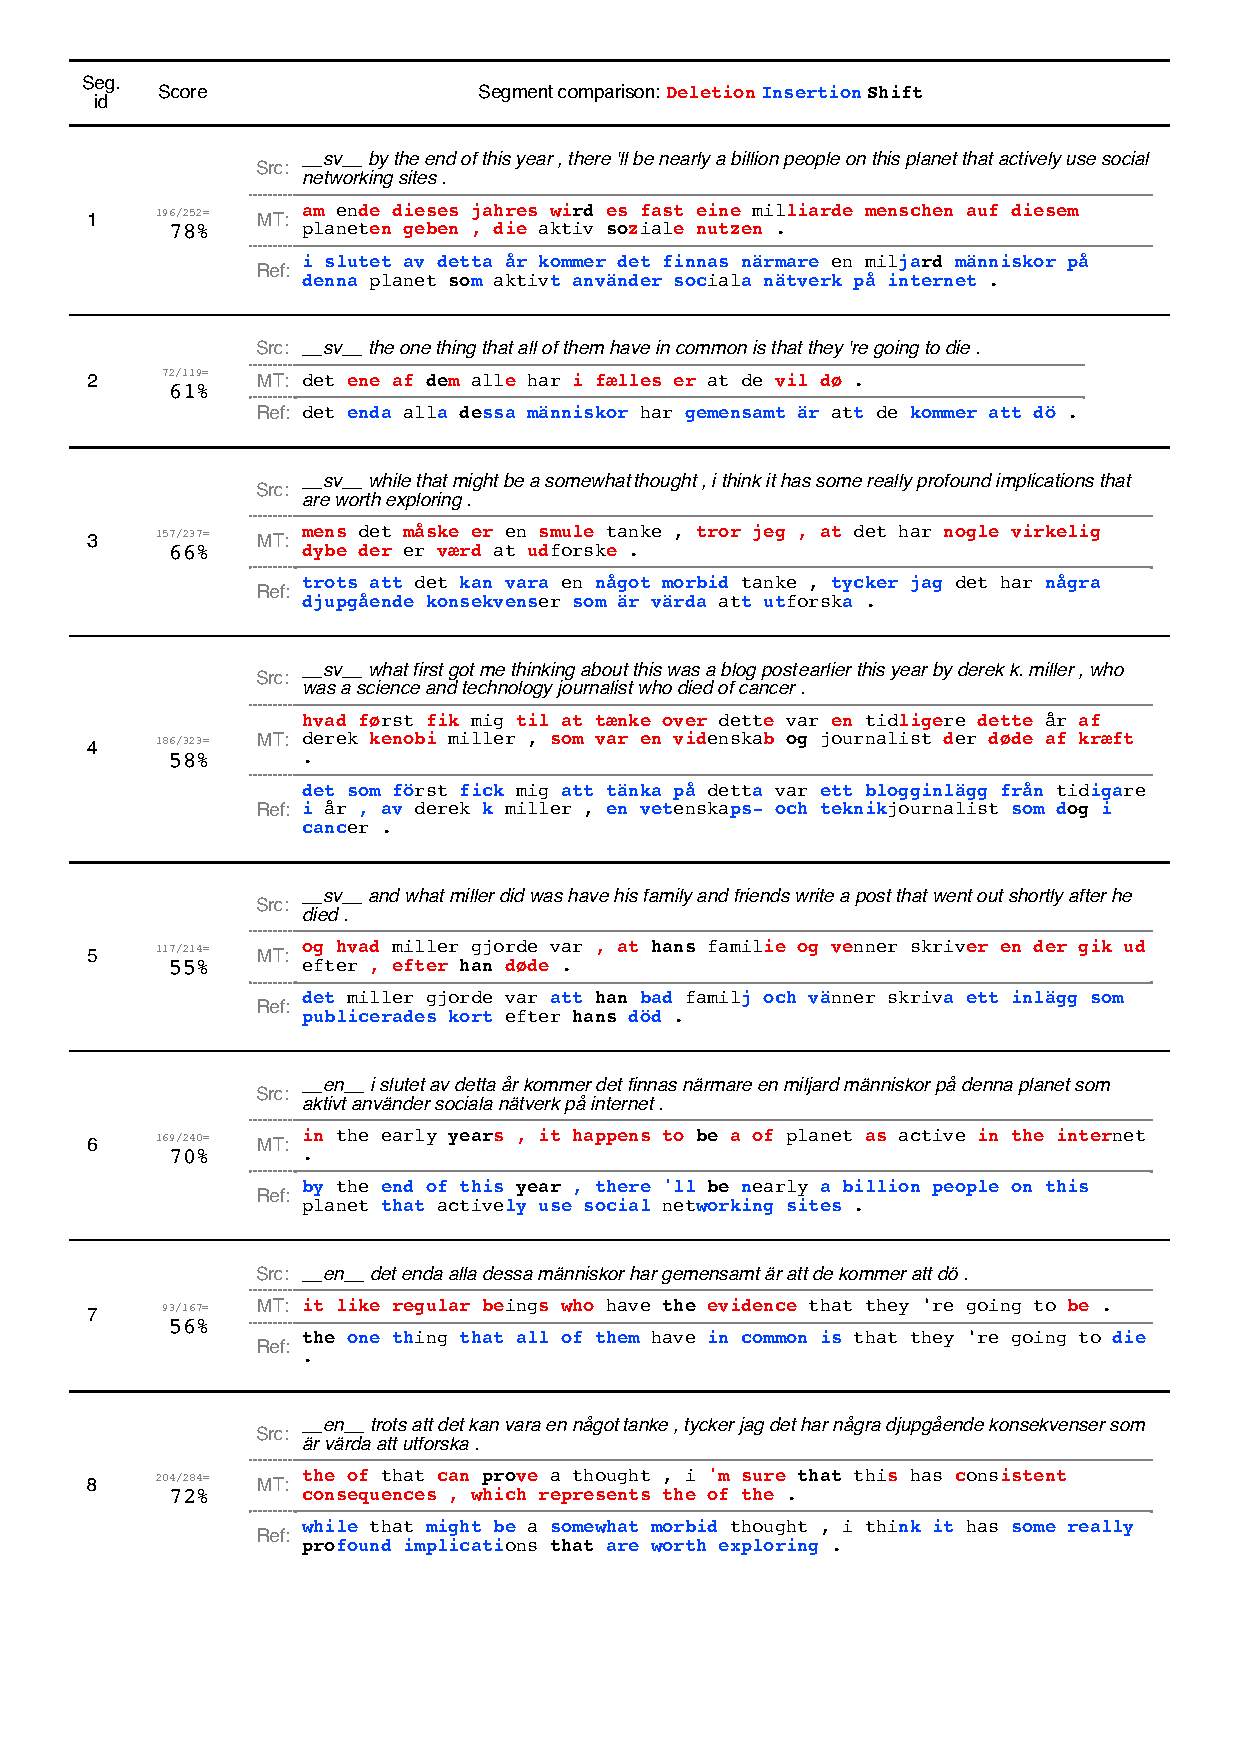
\includepdf[pages=-,scale=0.9,pagecommand={}]{mt_example_output/en+de+da+sv.pdf}

\printbibliography
\end{document}
